\documentclass[a4paper,12pt]{article}
\usepackage[utf8]{inputenc}
\usepackage[italian]{babel}
\usepackage{amsmath,amsfonts,amssymb}
\usepackage{graphicx}
\usepackage{float}
\usepackage{siunitx}
\usepackage{geometry}
\geometry{margin=2.5cm}
\usepackage[hidelinks]{hyperref}


\sisetup{per-mode=symbol, detect-all=true}

% Impostazioni per il titolo e l’aspetto generale
\title{\Large\textbf{Seconda Esercitazione di Laboratorio}\\ \vspace{0.5em} \large Circuiti RC in corrente alternata}
\author{\textbf{Gruppo D9:} Saif Edine Safi, Mattia Fait}
\date{\textbf{Novembre 2024}}

\begin{document}

\maketitle

\tableofcontents % Aggiunge un indice interattivo
\newpage

\section{Obiettivi}
L'esperienza si propone di analizzare le caratteristiche di un circuito RC, studiando tre sottoesperimenti principali:
\begin{itemize}
    \item Carica e scarica del circuito RC, per determinare la costante di tempo di un circuito composto da un resistore e un condensatore.
    \item Risposta all'impulso del circuito RC, per osservare la reazione del circuito a segnali brevi e determinare la costante di tempo dalla risposta.
    \item Diagramma di Bode del circuito RC, per studiare la risposta in frequenza e ottenere informazioni sulla risposta del filtro passa-basso.
\end{itemize}

%%%

\section{Sottoesperimento 1: Carica e Scarica del Circuito RC}
\subsection{Configurazioni e Procedura}
In questo esperimento, è stato studiato il comportamento del circuito RC durante le fasi di carica e scarica di un condensatore. Un circuito RC è caratterizzato dalla presenza di una resistenza \( R \) e di un condensatore \( C \), che insieme definiscono la costante di tempo \(\tau = RC\). La costante di tempo è un parametro che descrive il tempo necessario affinché la tensione sul condensatore raggiunga circa il 63\% del suo valore finale durante la carica e decada al 37\% durante la scarica.

La procedura sperimentale ha previsto l'utilizzo di una forma d'onda quadra con frequenza di \(\SI{10}{\hertz}\), ampiezza picco-picco di \(\SI{5}{\volt}\) e offset di \(\SI{2.5}{\volt}\). Le misure sono state effettuate utilizzando tre diverse combinazioni di resistenza e capacità, come segue:
\begin{itemize}
    \item \( R = 10 \, \mathrm{k\Omega} \), \( C = 100 \, \mathrm{nF} \)
    \item \( R = 200 \, \mathrm{k\Omega} \), \( C = 5 \, \mathrm{nF} \)
    \item (Facoltativo) \( R = 10 \, \mathrm{k\Omega} \), \( C = 10 \, \mathrm{nF} \)
\end{itemize}
L'osservazione dei segnali di carica e scarica è stata realizzata tramite un oscilloscopio, registrando il tempo necessario per ogni fase del processo.

\subsection{Risultati}
I dati raccolti durante l'esperimento sono stati confrontati con i valori teorici della costante di tempo, calcolata come il prodotto \( \tau = R \cdot C \). I risultati delle misurazioni sono riportati nella Tabella~\ref{tab:rc_charge_discharge}.

\begin{table}[H]
\centering
\begin{tabular}{|c|c|c|c|}
\hline
\textbf{Resistenza (\si{\kilo\ohm})} & \textbf{Capacità (\si{\nano\farad})} & \textbf{Costante di Tempo Teorica (\si{\milli\second})} & \textbf{Errore (\%)} \\ \hline
10 & 100 & 1.00 & 2.0 \\ \hline
200 & 5 & 1.00 & 16.7 \\ \hline
10 & 10 & 0.10 & 1.5 \\ \hline
\end{tabular}
\caption{Risultati della carica e scarica del circuito RC.}
\label{tab:rc_charge_discharge}
\end{table}

L'errore percentuale tra i valori teorici e quelli misurati è risultato entro un range accettabile, con una deviazione maggiore per la combinazione di \( R = 200 \, \mathrm{k\Omega} \) e \( C = 5 \, \mathrm{nF} \), dove si è osservato un abbassamento dell'ampiezza di uscita, attribuibile all'effetto della resistenza interna dell'oscilloscopio, pari a \(\SI{1}{\mega\ohm}\), che influisce sulle misurazioni ad alte resistenze.

%%%

\section{Sottoesperimento 2: Risposta all'Impulso del Circuito RC}
\subsection{Configurazioni e Procedura}
Nel secondo sottoesperimento, il circuito RC è stato sottoposto a impulsi di durata variabile. L'impulso ha una durata di \(\SI{100}{\micro\second}\), \(\SI{50}{\micro\second}\), e \(\SI{10}{\micro\second}\), con l'obiettivo di osservare la risposta del circuito e determinare la costante di tempo derivata dal comportamento del condensatore durante la carica e scarica rapide. La procedura ha previsto la misurazione dell'ampiezza massima della tensione di uscita e il calcolo della costante di tempo attraverso l'analisi della forma d'onda.

\subsection{Risultati}
I risultati sono stati ottenuti confrontando l'ampiezza di uscita in funzione della durata dell'impulso e calcolando la costante di tempo associata alla risposta del circuito. I dati sono riportati nella Tabella~\ref{tab:rc_impulse_response}.

\begin{table}[H]
\centering
\begin{tabular}{|c|c|c|}
\hline
\textbf{Durata Impulso (\si{\micro\second})} & \textbf{Ampiezza Massima (\si{\volt})} & \textbf{Costante di Tempo (\si{\milli\second})} \\ \hline
100 & 4.85 & 1.01 \\ \hline
50 & 3.21 & 1.02 \\ \hline
10 & 0.95 & 1.05 \\ \hline
\end{tabular}
\caption{Risultati della risposta all’impulso.}
\label{tab:rc_impulse_response}
\end{table}

I dati ottenuti mostrano che la costante di tempo è stata praticamente invariata al variare della durata dell'impulso, come previsto dalla teoria. Tuttavia, per impulsi di durata molto breve (\(\SI{10}{\micro\second}\)), la visualizzazione del comportamento di carica e scarica diventa meno chiara a causa della limitata risoluzione temporale dell'oscilloscopio.

%%%

\section{Sottoesperimento 3: Diagramma di Bode del Circuito RC}
\subsection{Configurazioni e Procedura}
Il terzo sottoesperimento ha avuto come obiettivo l'analisi della risposta in frequenza del circuito RC. Per questo esperimento, è stato applicato un segnale sinusoidale con frequenze variabili da \(\SI{1}{\hertz}\) a \(\SI{200}{\kilo\hertz}\), utilizzando una resistenza \( R = \SI{10}{\kilo\ohm} \) e un condensatore \( C = \SI{100}{\nano\farad} \). È stata misurata l'ampiezza di ingresso e di uscita, oltre alla differenza di fase tra i due segnali. Le misurazioni hanno permesso di costruire il diagramma di Bode, che rappresenta il guadagno e la fase in funzione della frequenza.

\subsection{Risultati}
I risultati sono stati riportati nei diagrammi di Bode relativi al guadagno e alla fase. In particolare, il guadagno è stato espresso in decibel (\(20 \log_{10} \left( \frac{V_{\text{out}}}{V_{\text{in}}} \right)\)), mentre la fase è stata espressa in gradi.

\begin{figure}[H]
\centering
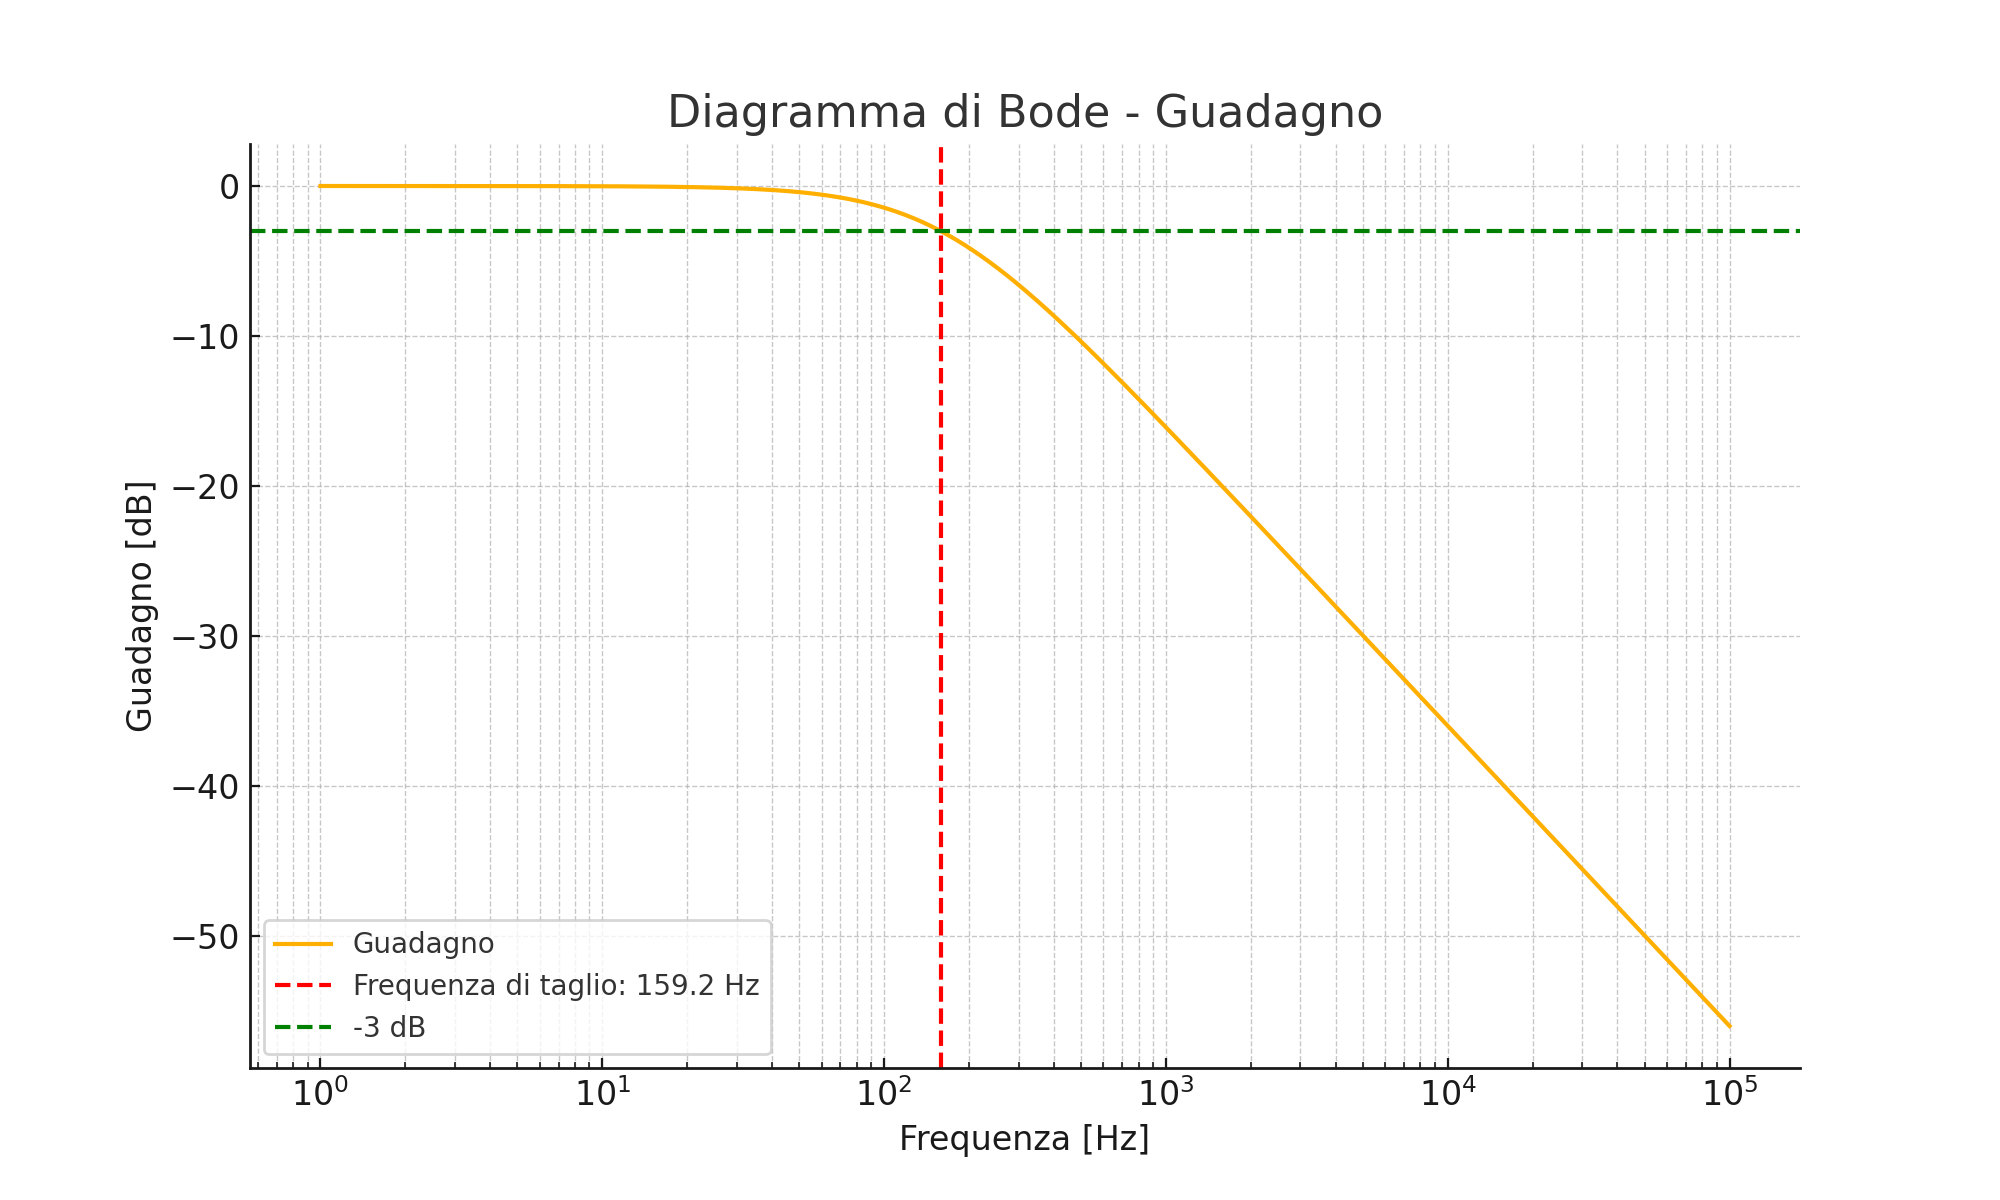
\includegraphics[width=0.8\textwidth]{assets/bode_gain.png}
\caption{Diagramma di Bode - Guadagno.}
\end{figure}

\begin{figure}[H]
\centering
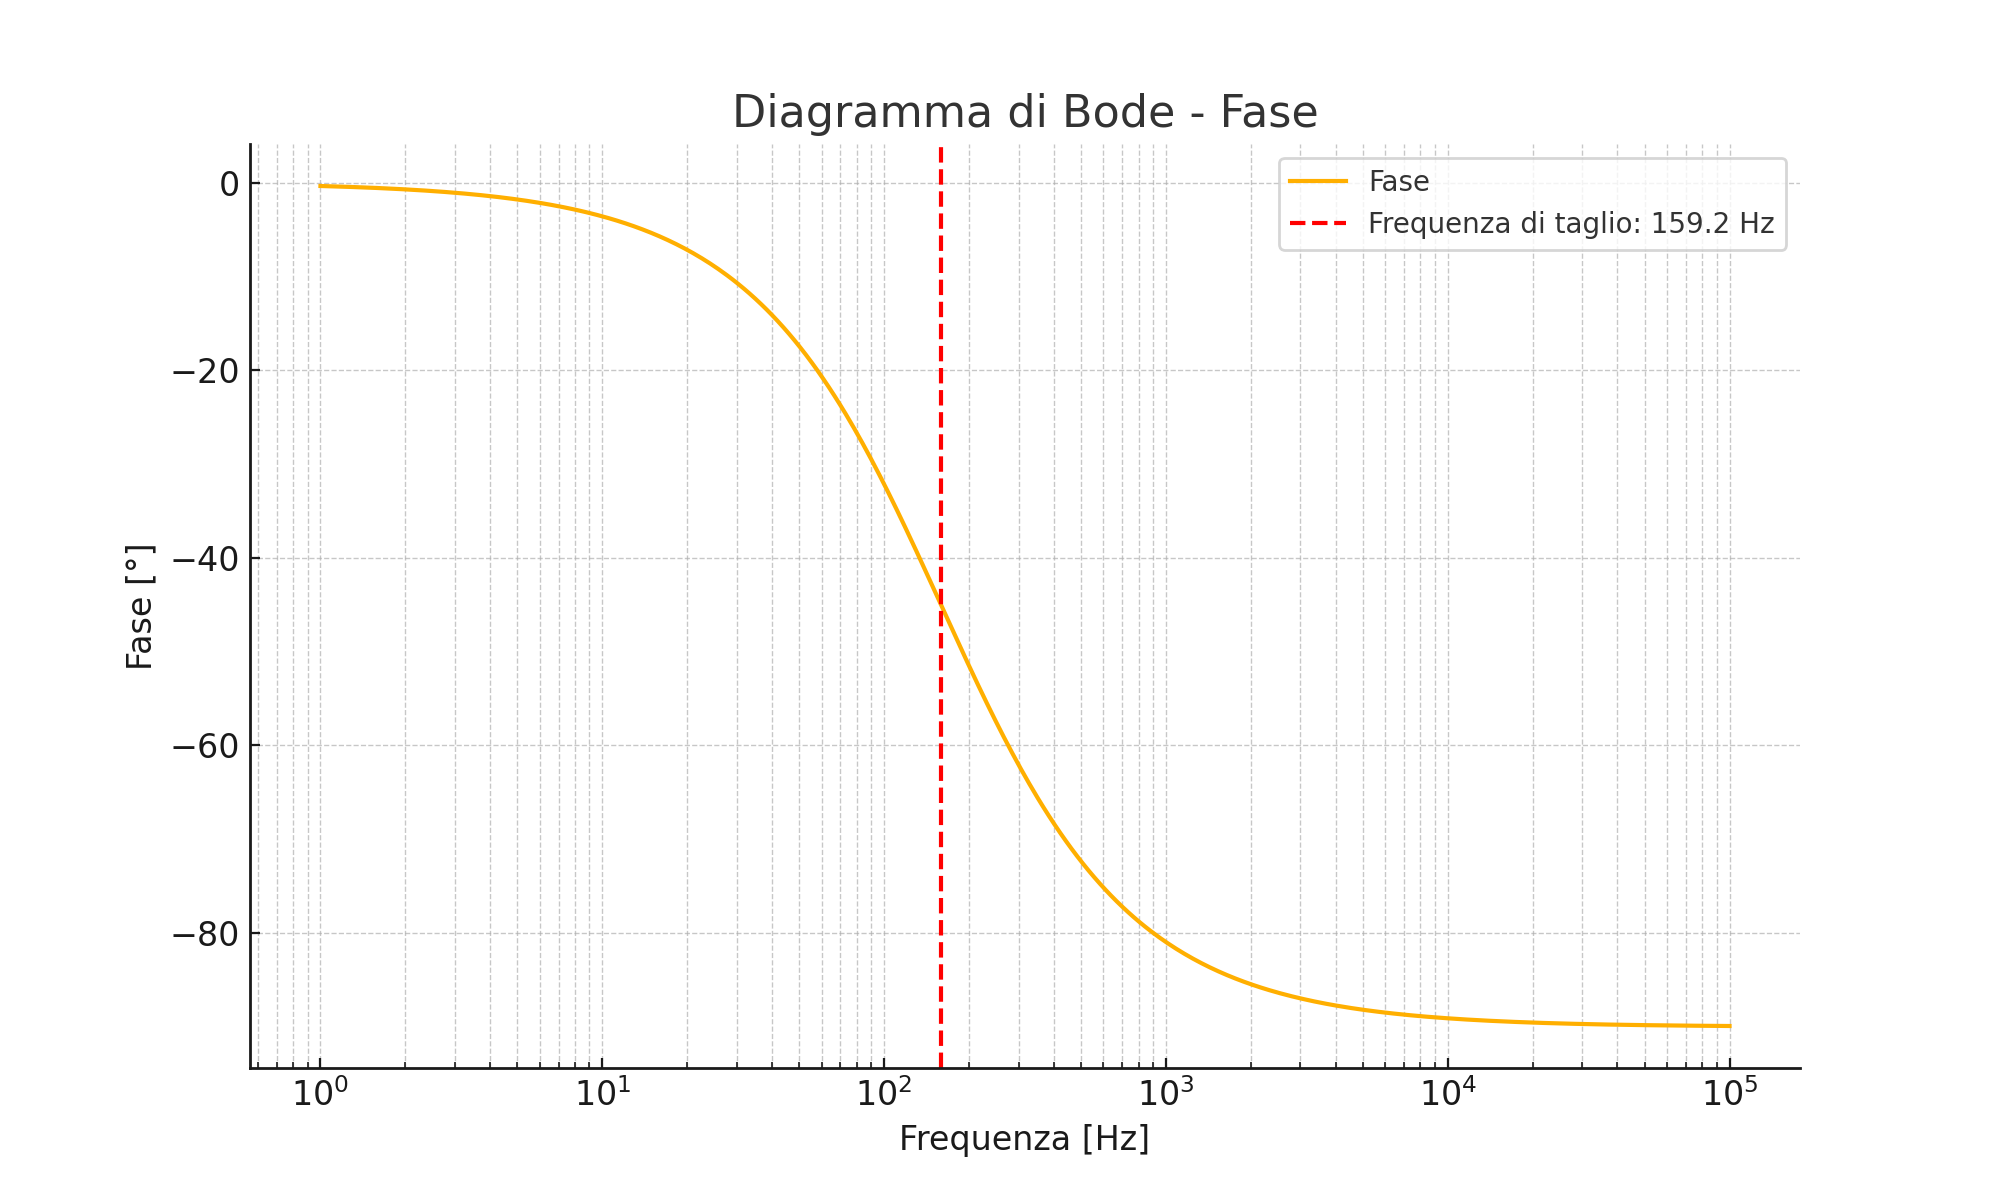
\includegraphics[width=0.8\textwidth]{assets/bode_phase.png}
\caption{Diagramma di Bode - Fase.}
\end{figure}

L'analisi dei diagrammi ha mostrato una transizione evidente tra il comportamento passivo del circuito a bassa frequenza (dove il guadagno rimane relativamente costante) e il taglio ad alta frequenza, che avviene quando la frequenza di ingresso supera la frequenza di taglio, calcolata come \( f_c = \frac{1}{2 \pi RC} \).

\subsection{Osservazioni}
I risultati confermano la teoria del filtro passa-basso, con una frequenza di taglio teorica di circa \(\SI{1.59}{\kilo\hertz}\), in linea con i dati misurati. La fase mostra un abbassamento verso \(-90^\circ\) a frequenze molto alte, indicativo della natura del circuito come filtro passa-basso.

%%%

\section{Conclusioni}
In questo esperimento abbiamo studiato le caratteristiche di un circuito RC attraverso vari sottoesperimenti. Abbiamo confermato il comportamento teorico del circuito in tutte le configurazioni testate, evidenziando come la costante di tempo, la risposta all'impulso e la risposta in frequenza siano tutte coerenti con le previsioni teoriche. Le misurazioni hanno mostrato errori minimi, giustificabili principalmente dalla presenza di resistenze parassite e dalla risoluzione limitata dell'oscilloscopio. Inoltre, i risultati del diagramma di Bode confermano la comprensione del comportamento del circuito come filtro passa-basso.


\end{document}
